\documentclass[review,hidelinks,onefignum,onetabnum]{siamart251216}
% Shared setup follows SIAM's ex_shared.tex.
\usepackage{amsfonts,amssymb,graphicx,booktabs}
\emergencystretch=1em
\newsiamremark{remark}{Remark}
\headers{Minimum central circles}{M. Falconi}
\title{The minimum central circle for prescribed radius profiles\thanks{An earlier version appeared as
\href{https://arxiv.org/abs/2609.13630v3}{arXiv:2609.13630v3}.}}
\author{Maurizio Falconi\thanks{Independent researcher, Parma, Italy
(\email{maurizio.falconi47@gmail.com}).}}
\hypersetup{pdfauthor={Maurizio Falconi}}
\pdfinfoomitdate=1
\pdftrailerid{}
\pdfsuppressptexinfo=15

% Certified decimal bounds for the limiting ring coefficients.
\newcommand{\CstarLower}{0.1405694688}
\newcommand{\CstarUpper}{0.140958576058}
\newcommand{\CtwoUpper}{0.088581212993}

\hypersetup{pdftitle={The minimum central circle for prescribed radius profiles}}
\externaldocument[s1-][nocite]{supplement}
\newcommand{\Rstar}{R^\ast}
\newcommand{\ch}{R_{\mathrm{chain}}}
\newcommand{\full}{R_{\mathrm{full}}}
\newcommand{\CC}{C_\ast}
\DeclareMathOperator{\atan}{arctan}
\DeclareMathOperator{\asin}{arcsin}
\begin{document}
\maketitle
\begin{abstract}
Let $R_n$ be the infimum radius of a central circle externally tangent
to $n$ disks with pairwise disjoint interiors. Write the outer radii as
$N_n a_{n,i}$, with positive scales $N_n$ and uniformly bounded
nonnegative marks. If the empirical laws of the marks converge weakly
to $\mu$, then $R_n/(N_n n)\to E(\mu)/\pi$. Here $E(\mu)$ is the limiting
mean span of points on a line whose pairwise separations are at least the
geometric means of their marks. A linear program on $k$ quantile types
and words of length $r$ encloses the limiting ring coefficient within an
interval of width $M(k+r)/(\pi kr)$ before numerical evaluation of the
word costs, where $M$ is the common mark bound.
For consecutive integer radii the minimum grows quadratically, with leading
coefficient $0.1405694688<C_\ast<0.140958576058$. Coupled terminal subsets give
the lower bound and a rational line placement gives the upper bound. The
profile theorem also applies to every fixed positive power of the labels.
For square radii the growth is cubic, with leading coefficient less than
$0.088581212993$.
\end{abstract}
\begin{keywords}
circle packing, geometric optimization, asymptotic limits, linear programming,
rigorous computation
\end{keywords}
\begin{MSCcodes}
52C15, 52C26, 90C05
\end{MSCcodes}

\section{The minimum central circle}

Consider $n$ disks externally tangent to a central circle, with pairwise
disjoint interiors. Write their prescribed radii as $N_n a_{n,i}$, with
scale $N_n>0$ and marks $a_{n,i}\in[0,M]$ for a fixed $M<\infty$.
We minimize the central radius over all orders and placements. Our main
example has $N_n=n$ and $a_{n,i}=i/n$, so the outer radii are
$1,\ldots,n$ and their normalized distribution tends to the uniform law.
For this example, write $\full(\sigma)$ for the least feasible radius
in cyclic order $\sigma$ and $\Rstar(n)=\min_\sigma\full(\sigma)$.
The adjacent-chain closure $\ch(\sigma)$ bounds $\full(\sigma)$ from
below. Paper~I~\cite{paperI} treats these chains and certifies tight
global brackets for $3\le n\le14$.

\paragraph*{Main results}
\begin{enumerate}
\item If the empirical laws of the marks converge weakly to $\mu$, the
normalized radius converges to $E(\mu)/\pi$
(Theorem~\ref{thm:profile-law}). A stability estimate for the square
roots of matched marks allows atoms and zero radii. For $k$ quantile
types and words of length $r$, Theorem~\ref{thm:profile-words} bounds
the limiting coefficient within an interval of width $M(1/k+1/r)/\pi$.
\item For consecutive integer radii,
$\Rstar(n)=\CC n^2+o(n^2)$. Theorems~\ref{thm:existence}
and~\ref{thm:lp} give the finite-template infimum and the uniform
finite-word program. Proposition~\ref{prop:lower} and the certificate
in Proposition~\ref{prop:cert-upper} give $\CstarLower<\CC<\CstarUpper$.
In particular the lower endpoint excludes the coefficient $1/8$ proposed
in the first version of Paper~I~\cite{paperI}.
\item For each fixed $p>0$, radii $i^p$ have a leading term
$C_p n^{p+1}$ (Corollary~\ref{cor:profile-powers}). For square radii,
the adjacent-pair bound and the second line certificate give
$1/(6\pi)\le C_2<\CtwoUpper$.
\end{enumerate}

\paragraph*{Related work}
Alt et al.~\cite{shelf} study disks resting on a shelf and minimizing
the width of their horizontal envelope. Their geometric-mean separation
rule gives the line problem in Definition~\ref{def:line} (Figure~\ref{fig:line}).
For marks at most one, that envelope differs from
$2(\max_i x_i-\min_i x_i)$ by at most two.
Klemz, N\"ollenburg and Prutkin~\cite{contact} study weighted disk
contact graphs, where a prescribed graph specifies the tangencies. In
the central-circle problem all spokes are required and the outer
contacts are free. For a fixed order, angular feasibility has a
difference-constraint formulation in Paper~I, in the framework of
temporal constraint networks~\cite{temporal}. The chain-order result
of Paper~I uses Supnick's structured traveling-salesman
problem~\cite{supnick}, part of the class of tractable cases surveyed
by Burkard et al.~\cite{burkard}.

The shortest-tour theorem of Beardwood, Halton and Hammersley~\cite{bhh}
also identifies a leading geometric optimization constant, for randomly
sampled points. Steele~\cite{steele} develops probabilistic approaches
to combinatorial optimization. Here every size has its own deterministic
set of labels. The finite-type argument uses the elementary subadditivity
lemma~\cite[Theorem~4.9]{walters}, while the passage between different
label sets requires reassignment in Theorem~\ref{thm:existence}.
The use of verified arithmetic for finite inequalities follows the
distinction between numerical approximation and certified bounds
developed by Rump~\cite{rump} and Tucker~\cite{tucker}.

\section{Exact Angular Comparison}\label{sec:line}

The cosine law gives the required pair angle
\begin{equation}\label{eq:theta}
 \theta_R(u,v)=2\asin\sqrt{\frac{uv}{(R+u)(R+v)}}
 =2\atan\sqrt{\frac{uv}{R(R+u+v)}}.
\end{equation}
Both directed cyclic arcs between a pair must be at least this angle.
This is equivalent to non-overlap, since their smaller separation belongs
to $[0,\pi]$. For positive outer radii the angle is positive, symmetric, increasing in either
outer radius and strictly decreasing in $R>0$.
For a cyclic order $\sigma=(u_1,\ldots,u_n)$ of positive radii, $n\ge3$, with $u_{n+1}=u_1$,
$\ch(\sigma)$ is the unique positive root of
$\sum_{i=1}^n\theta_R(u_i,u_{i+1})=2\pi$.
Indeed, the sum decreases continuously from $n\pi$ to zero. Summing the
adjacent constraints in any full placement proves $\ch(\sigma)\le\full(\sigma)$.

We next introduce an auxiliary problem on a line. Its comparison with the
circle problem will follow after a bound on the cost of closing a line
placement.

\begin{definition}\label{def:line}
For a finite multiset $a=(a_1,\ldots,a_N)$ of marks in $[0,1]$, let $b(a)$
be the least span of a line placement satisfying
\begin{equation}\label{eq:line}
 |x_i-x_j|\ge\sqrt{a_i a_j}\quad(i\ne j).
\end{equation}
Distinct zero-mark points may coincide. Write $b_n=b(1/n,2/n,\ldots,1)$.
\end{definition}

\begin{figure}[tb]
\centering
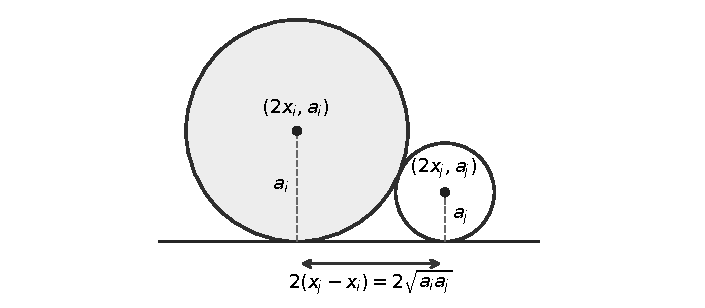
\includegraphics[width=.65\linewidth]{figures/line_geometry.pdf}
\caption{Two disks tangent to the same line. Their center separation
squared is $4(x_j-x_i)^2+(a_j-a_i)^2$. At contact this equals
$(a_i+a_j)^2$, giving equality in~\eqref{eq:line}.}
\label{fig:line}
\end{figure}

For a fixed word $w=(w_1,\ldots,w_N)$ in left-to-right order, its minimum
span $\ell(w)$ is attained by
\begin{equation}\label{eq:recurrence}
 x_1=0,\qquad x_i=\max_{j<i}\{x_j+\sqrt{w_iw_j}\},\qquad \ell(w)=x_N.
\end{equation}
Induction proves that these coordinates are componentwise no larger than
any feasible ordered coordinates with $x_1=0$; they also satisfy every
constraint. Nonnegative weights ensure ordered coordinates. Equivalently,
$\ell(w)$ is the longest increasing-index path from $1$ to $N$, with
edge weight $\sqrt{w_iw_j}$. Thus $b(a)$ is an attained minimum over a
finite set of orders. Deleting or decreasing marks cannot increase it;
scaling all marks by $h$ scales the minimum span by $h$.

\begin{lemma}[Bounded closing cost]\label{lem:closing}
Let $B(a)$ be the infimum circumference with both pair arcs at least
$\sqrt{a_i a_j}$. Then $b(a)\le B(a)\le b(a)+1$.
\end{lemma}
\begin{proof}
Cut a feasible circle to obtain a feasible line placement. Conversely,
close a feasible line placement by an additional gap of length one. One
arc for every pair is its line separation; the other contains the added
gap and is at least $1\ge\sqrt{a_i a_j}$. Both arcs are controlled.
\end{proof}

\begin{lemma}[Exact geometric squeeze]\label{lem:squeeze}
For every $n\ge3$,
\begin{equation}\label{eq:squeeze}
 \frac{b_n}{\pi n}-\frac1n
 \le\frac{\Rstar(n)}{n^2}\le\frac{b_n+1}{\pi n}.
\end{equation}
\end{lemma}
\begin{proof}
For $1\le u,v\le n$, the two expressions in \eqref{eq:theta} give
\[
 \frac{2\sqrt{uv}}{R+n}\le\theta_R(u,v)\le\frac{2\sqrt{uv}}R.
\]
The first uses $\asin z\ge z$ and
$\sqrt{(R+u)(R+v)}\le R+n$; the second uses $\atan z\le z$.
Scaling a feasible ring's angles by $(R+n)/(2n)$ gives a feasible linear
circle of circumference $\pi(R+n)/n$, proving the lower inequality.
Conversely, the circumference $b_n+1$ from Lemma~\ref{lem:closing},
scaled to $2\pi$, satisfies every original pair angle at
$R=n(b_n+1)/\pi$. This proves the upper inequality. No Taylor expansion,
adjacency reduction or assumption on the optimal order was used.
\end{proof}

\section{Existence by Genuine-Label Concatenation}

The closing estimate makes concatenation useful: copies of a finite line
placement can be joined at bounded cost. The next theorem combines this
construction with reassignment to the prescribed normalized radii.

\begin{theorem}[The leading limit exists]\label{thm:existence}
There is a constant $\CC$ such that
\begin{equation}\label{eq:limit}
 \Rstar(n)=\CC n^2+o(n^2),\qquad
 \pi\CC=E:=\lim_{n\to\infty}\frac{b_n}{n}
 =\inf_{n\ge2}\frac{b_n+1}{n}.
\end{equation}
\end{theorem}
\begin{proof}
Copies of a feasible line template, separated by unit gaps, satisfy all
cross-copy constraints as well as the internal ones. Fix $n\ge2$. Given
$N\ge n$, let $q=\lceil N/n\rceil$ and concatenate $q$ copies of an
optimal $b_n$ template. Its span is $q(b_n+1)-1$.
Retain the $N$ smallest marks. The $i$th sorted retained mark is
$\lceil i/q\rceil/n$. Scale all marks and coordinates by $h=nq/N$.
The resulting $i$th mark is at least $i/N$, so decreasing it to $i/N$
preserves every constraint. Each target label is assigned exactly once
to an actual retained point, with ties broken arbitrarily. Hence
\begin{equation}\label{eq:copies}
 b_N\le\frac{nq}{N}\bigl[q(b_n+1)-1\bigr].
\end{equation}
Intermediate marks exceeding one cause no problem: the line inequalities
are homogeneous, and final marks are exactly $1/N,\ldots,1$.

As $N\to\infty$, $q/N\to1/n$, giving
$\limsup_N b_N/N\le(b_n+1)/n$ for every fixed $n$.
The sequence is bounded between zero and one by equally spaced placements.
Taking $n$ along a subsequence attaining its liminf gives equality of
limsup and liminf. Taking the infimum and then $n\to\infty$ proves
the last equality in \eqref{eq:limit}. Lemma~\ref{lem:squeeze} transfers
the limit to the original ring problem for all sizes and both parities.
Finally, at least $n/2$ marks are at least $1/2$. Their successive line
separations are at least $1/2$, so $E\ge1/4$ and $\CC>0$.
\end{proof}

\section{A finite linear-programming characterization}\label{sec:lp}

We now turn from existence of the limit to approximation with a prescribed
error. There are two steps: replace the radii by finitely many types, then
replace long orderings by distributions of finite words. Each step contributes
one term to the bracket width.

\subsection{Finite Types and a Uniform Quantization Error}
For $k\ge1$, let $A_{k,q}$ contain $q$ copies of each mark
$1/k,\ldots,1$, and let $A^-_{k,q}$ instead contain $q$ copies of
$0,1/k,\ldots,(k-1)/k$. Define
$e_k=\lim_{q\to\infty}b(A_{k,q})/(kq)$ and
$e^-_k=\lim_{q\to\infty}b(A^-_{k,q})/(kq)$; these limits exist.
Indeed $a_q=b(A_{k,q})+1$ is subadditive by unit-gap concatenation.
Writing $q=hp+s$ at fixed $p$ proves
$\limsup a_q/q\le a_p/p$; then taking $p$ along a liminf subsequence
proves the limit. The same argument applies to the lower types.

The two multisets share every nonzero type except the top type. Zero marks
cost nothing. Adding the $q$ unit marks as a separate equally spaced
block costs at most $q$, including the join. Thus, also for $k=1$,
\[
 e^-_k\le e_k\le e^-_k+\frac1k.
\]
For $n=kq$, the sorted uniform marks $i/n$ lie between the two sorted
type multisets. Theorem~\ref{thm:existence} and monotonicity imply
\begin{equation}\label{eq:types}
 e_k-\frac1k\le E\le e_k.
\end{equation}

\subsection{Balanced Words and the Quantified Boundary Relaxation}
A word records a short consecutive piece of an ordering. The linear program
balances type counts across a distribution of words; the proof below controls
the cost of joining them.

Fix $k\ge1$ and $r\ge2$, and use all $k^r$ words
$w\in\{1/k,\ldots,1\}^r$, including repetitions. Let $c_j(w)$ count
occurrences of $j/k$. Compute $\ell(w)$ by \eqref{eq:recurrence}, and define
\begin{equation}\label{eq:lp}
\begin{split}
 \lambda_{k,r}=\min_p\ &\frac1r\sum_w p_w\ell(w),\\
 p_w\ge0,\quad &\sum_w p_w=1,\quad
 \sum_w p_wc_j(w)=\frac rk\quad(1\le j\le k).
\end{split}
\end{equation}
The polytope is nonempty: equally mix the $k$ constant words.

\begin{theorem}[Finite linear-programming bounds]\label{thm:lp}
For every $k\ge1,r\ge2$,
\begin{equation}\label{eq:effective}
 \boxed{\quad\frac{\lambda_{k,r}-1/k}{\pi}\le\CC
 \le\frac{\lambda_{k,r}+1/r}{\pi}\quad}.
\end{equation}
Consequently $\CC=\pi^{-1}\lim_{k,r\to\infty}\lambda_{k,r}$, jointly,
with certified bracket width $(1/k+1/r)/\pi$.
\end{theorem}
\begin{proof}
Partition an optimal ordering of $A_{k,q}$ into consecutive blocks of
$r$ vertices, discarding fewer than $r$ leftover vertices. Their spans
sum to at most the full span and each is at least its word cost.
Empirical word distributions have convergent subsequences in the finite
simplex. Their limiting mean type counts are $r/k$, since the discarded
counts vanish after normalization. Hence $\lambda_{k,r}\le e_k$.

Conversely, the rational feasible polytope in \eqref{eq:lp} has a minimizing
rational vertex even though its cost entries are algebraic. Choose a
common denominator $D$. A batch with $Dp_w$ copies of each word has
exactly $Dr/k$ copies of each type, an integer by the count constraints.
Place every word at its minimum span and separate blocks by unit gaps.
All within-block and cross-block pairs are feasible. Repeating batches
gives asymptotic mean span
$\sum_w p_w(\ell(w)+1)/r=\lambda_{k,r}+1/r$.
The finite-type limit therefore satisfies
$e_k\le\lambda_{k,r}+1/r$. Combine with \eqref{eq:types}.
\end{proof}

\subsection{Exact Certificates and Computational Meaning}
Directed rational square-root enclosures of width $\epsilon$ give
word-span enclosures of width at most $(r-1)\epsilon$: every path in
\eqref{eq:recurrence} has at most $r-1$ edges. Rational endpoint LPs
then enclose $\lambda_{k,r}$ with additional width at most
$(r-1)\epsilon/r$. They can be solved by finite exact vertex enumeration.
Practical solvers may instead find solutions for subsequent exact verification.
For a rational lower cost $\ell^-(w)$, dual coefficients satisfying
\[
 y_0+\sum_j y_jc_j(w)\le\ell^-(w)/r\quad\hbox{for every word}
\]
certify the lower value $y_0+(r/k)\sum_jy_j$. Feasible rational $p$
certifies an upper value using upper costs. All such checks are finite
rational comparisons; equality is not decided by indefinite interval
refinement. Together with a rational enclosure of $\pi$, this proves
arbitrary-precision computability of $\CC$ in principle.

For example, $k=r=64$ gives width $1/(32\pi)<0.01$ before directed
arithmetic error, with $64^{64}$ words in the displayed formulation.
For the uniform profile the explicit endpoint bounds below bypass this enumeration.

\section{Prescribed radius profiles}\label{sec:profiles}

Let $a_n=(a_{n,1},\ldots,a_{n,n})$ be a list of marks in $[0,M]$,
where $M<\infty$ is independent of $n$. Write $R_n$ for the infimum
central radius for outer radii $N_n a_{n,i}$, with $N_n>0$. A zero mark
represents a point on the central circle and imposes no separation.
Use $b(a_n)$ for the least span under the same geometric-mean constraints
as in~\eqref{eq:line}. The recurrence~\eqref{eq:recurrence} applies to
these marks, with no change of units.

\begin{lemma}[Geometric comparison for bounded marks]\label{lem:profile-squeeze}
For $n\ge3$,
\begin{equation}\label{eq:profile-squeeze}
 \frac{b(a_n)}{\pi n}-\frac{M}{n}
 \ \le\ \frac{R_n}{N_n n}\ \le\ \frac{b(a_n)+M}{\pi n}.
\end{equation}
\end{lemma}
\begin{proof}
For $u,v\le N_nM$ and $R>0$, \eqref{eq:theta} gives
$2\sqrt{uv}/(R+N_nM)\le\theta_R(u,v)\le2\sqrt{uv}/R$.
Scale both arcs of a feasible ring by $(R+N_nM)/(2N_n)$ and cut
the ring. The resulting line placement has span at most $\pi(R/N_n+M)$.
Conversely, join the ends of a minimizing line placement with a gap $M$.
Each pair has its line separation on one arc and the gap on the other.
Scaling the circumference $b(a_n)+M$ to $2\pi$ gives full feasibility
at $R=N_n(b(a_n)+M)/\pi$. If $M=0$, the infimum is zero.
\end{proof}

\subsection{From a quantile template to a limit law}

For a nondecreasing function $Q:(0,1]\to[0,M]$, write
$b_n^Q=b(Q(1/n),\ldots,Q(1))$. For a probability law $\mu$ on $[0,M]$,
its quantile is $Q_\mu(t)=\inf\{x\in[0,M]:\mu([0,x])\ge t\}$,
$0<t\le1$.

\begin{lemma}[Replication of a quantile template]\label{lem:profile-copy}
If $m\ge n\ge2$ and $q=\lceil m/n\rceil$, then
\[
 b_m^Q\le q(b_n^Q+M)-M,\qquad
 \lim_{m\to\infty}\frac{b_m^Q}{m}=\inf_{n\ge2}\frac{b_n^Q+M}{n}.
\]
\end{lemma}
\begin{proof}
Place $q$ optimal copies with gaps $M$ and discard the $d=nq-m$
smallest donors. The $i$th remaining mark in sorted order has argument
$\lceil(i+d)/q\rceil/n\ge i/m$, because $m(i+d)-nqi=d(m-i)\ge0$.
Replace it by $Q(i/m)$. This assigns every target once and preserves
all separations, including for tied marks. At fixed $n$ the span bound
gives $\limsup_m b_m^Q/m\le(b_n^Q+M)/n$. The infimum of the right side
is at most $\liminf_n b_n^Q/n$, since $M/n\to0$ and
$0\le b_n^Q\le(n-1)M$.
\end{proof}

Denote the limit in Lemma~\ref{lem:profile-copy} for $Q=Q_\mu$ by $E(\mu)$.

\begin{theorem}[Radius-profile limit]\label{thm:profile-law}
If $n^{-1}\sum_{i=1}^n\delta_{a_{n,i}}$ converges weakly to $\mu$, then
\[
 \frac{b(a_n)}{n}\longrightarrow E(\mu),\qquad
 \frac{R_n}{N_n n}\longrightarrow\frac{E(\mu)}{\pi}.
\]
For a Riemann-integrable profile $f:[0,1]\to[0,M]$ sampled at $i/n$,
the limit law is that of $f(U)$, where $U$ is uniform on $(0,1)$.
\end{theorem}
\begin{proof}
For two matched lists $a,c$ of $n$ marks in $[0,M]$,
\begin{equation}\label{eq:profile-change}
 |b(a)-b(c)|\le2\sqrt M\sum_i|\sqrt{a_i}-\sqrt{c_i}|.
\end{equation}
Indeed, each edge product changes by at most $\sqrt M$ times the sum
of the changes in its endpoint square roots. A path uses each vertex
at most twice as an endpoint. Take the longest path in each fixed word
as in~\eqref{eq:recurrence}, then minimize over the orders.

Match the sorted square roots of $a_n$ to those of $Q_\mu(i/n)$.
Their mean absolute difference equals the integral over $[0,\sqrt M]$
of the absolute difference of the two empirical distribution functions.
At each threshold the two sorted indicator lists are nested, so
integrating their count difference gives the sum of the matched distances
after normalization. At threshold $s$, the quantile sample counts
$\lfloor n\mu([0,s^2])\rfloor$ entries. Its distribution function is
therefore within $1/n$ of that of $\sqrt{Q_\mu(U)}$. The distribution
functions of the array converge to that same function at its continuity
points. Bounded convergence gives a vanishing mean distance. Now
apply~\eqref{eq:profile-change}, Lemma~\ref{lem:profile-copy}
and~\eqref{eq:profile-squeeze}. For a Riemann-integrable profile, the
right-endpoint sums of each continuous test function composed with $f$
converge to its integral, giving the stated weak convergence.
\end{proof}

Applying~\eqref{eq:profile-change} to quantile samples and taking their
Riemann-sum limit gives, for laws $\mu,\nu$ on $[0,M]$,
\[
 |E(\mu)-E(\nu)|\le2\sqrt M
 \int_0^1|\sqrt{Q_\mu(t)}-\sqrt{Q_\nu(t)}|\,dt .
\]
Both quantiles are bounded and monotone, so the integrand is Riemann
integrable. In the uniform example $Q_\mu(t)=t$, Lemma~\ref{lem:profile-copy}
recovers the finite-template infimum for $\pi\CC$ in~\eqref{eq:limit}.

\subsection{Finite words and power radii}

Put $Q=Q_\mu$ and set $Q(0)=0$. Use the $k$ indexed types $v_j=Q(j/k)$,
retaining separate indices even if some values agree. Let
$\lambda_{k,r}(\mu)$ denote the program~\eqref{eq:lp} with these
types, where $\ell(w)$ uses the actual marks and $c_j(w)$ counts index $j$.

\begin{theorem}[Finite-word bounds for a law]\label{thm:profile-words}
For $k\ge1$ and $r\ge2$,
\[
 \lambda_{k,r}(\mu)-M/k\ \le\ E(\mu)\ \le\ \lambda_{k,r}(\mu)+M/r.
\]
The resulting bracket for $E(\mu)/\pi$ has width $M(1/k+1/r)/\pi$
before numerical evaluation of the type costs.
\end{theorem}
\begin{proof}
Let $e^+$ and $e^-$ be the limiting spans per mark for $q$ copies of
each upper type $Q(j/k)$ and each lower type $Q((j-1)/k)$, respectively,
as $q\to\infty$. These limits exist by Theorem~\ref{thm:profile-law}.
The sorted quantile grid of size $kq$ lies between the two lists.
Deleting the $q$ extra zeros in the lower list and appending $q$ top
marks costs at most $qM$, including the join. This also holds when the
common list is empty. Thus $e^+-M/k\le e^-\le E(\mu)\le e^+$.

Cut an optimal upper-type word into consecutive words of length $r$.
Their minimum spans sum to at most the full span. Fewer than $r$ leftover
marks are discarded, so a subsequential limit of the word distributions
has mean count $r/k$ for each index. This gives $\lambda_{k,r}(\mu)\le e^+$.
Conversely, the rational feasible polytope in~\eqref{eq:lp} contains the
uniform mixture of constant words and has a minimizing rational vertex,
even when the costs are real. A common denominator $D$ yields $D$ words
with exactly $Dr/k$ copies of each index. Repeat the batch with gaps $M$
between successive words. All pairs are feasible and the asymptotic cost
per mark is $\lambda_{k,r}(\mu)+M/r$, an upper bound on $e^+$.
\end{proof}

\begin{corollary}[Adjacent-pair lower bound]\label{cor:profile-adjacent}
For any probability law on $[0,M]$,
\[
 E(\mu)\ge\int_0^1\sqrt{Q_\mu(t)Q_\mu(1-t)}\,dt .
\]
\end{corollary}
\begin{proof}
Let $s_1\le\cdots\le s_n$ be the sorted square roots of the quantile
sample. In a feasible line order, successive gaps dominate the adjacent
products. Adding the closing product costs at most $M$. The cyclic
successor map permutes the square roots, so the rearrangement inequality
bounds the cyclic sum below by $\sum_i s_i s_{n+1-i}$. Hence the span
is at least this sum minus $M$. After division by $n$, the reverse-paired
sum converges to the displayed integral by bounded convergence, since
$Q_\mu$ is continuous at both $t$ and $1-t$ for almost every $t$.
\end{proof}

\begin{corollary}[Power radii]\label{cor:profile-powers}
For fixed real $p>0$ and outer radii $i^p$,
\[
 R_p^*(n)=C_p n^{p+1}+o(n^{p+1}),\qquad
 C_p=E(\operatorname{law}(U^p))/\pi .
\]
For square radii, $C_2\ge 1/(6\pi)$.
\end{corollary}
\begin{proof}
Take $N_n=n^p$ and $a_{n,i}=(i/n)^p$ in Theorem~\ref{thm:profile-law}.
The quantile is $Q(t)=t^p$. For $p=2$ the integral in
Corollary~\ref{cor:profile-adjacent} is $\int_0^1 t(1-t)\,dt=1/6$.
\end{proof}

\section{A certified upper bound}\label{sec:upper}

\begin{proposition}\label{prop:cert-upper}
The leading coefficients for consecutive integer radii and for square
radii satisfy, respectively,
\[
 \CC<\CstarUpper,\qquad C_2<\CtwoUpper .
\]
\end{proposition}
\begin{proof}
Write $Q_p(t)=t^p$ and $C_1=\CC$. By~\eqref{eq:limit} for $p=1$, and
by Lemma~\ref{lem:profile-copy} and Corollary~\ref{cor:profile-powers}
for $p=2$, $\pi C_p=\inf_{m\ge2}(b_m^{Q_p}+1)/m$.
Take $m=3200$. For each profile the certificate gives an integer
coordinate $X_i$ for each label. The following are the denominator $D$,
the span numerator $H=\max_i X_i-\min_i X_i$, and the strict decimal
ceiling $B$.
\[
\begin{array}{c r r l}
 p & D & H & B\\ \hline
 1 & m\,10^{12} & 4\,531\,424\,532\,506\,678\,377 & \CstarUpper\\
 2 & m^2 & 9\,108\,638\,531 & \CtwoUpper
\end{array}
\]
For every $i<j$, integer comparisons give
$m^2(X_i-X_j)^2\ge ijD^2$ for $p=1$ and
$m^2|X_i-X_j|\ge ijD$ for $p=2$. Thus $X_i/D$ realizes all required
separations and $b_m^{Q_p}\le H/D$. Using a rational lower bound for
$\pi$ from the alternating series in Machin's formula, the verifier checks
$(H/D+1)/(\pi m)<B$ in each case. The infimum formula gives the two
strict upper bounds.
\end{proof}

\begin{remark}
Reflected-block constructions with full geometric recovery appear in
arXiv:2609.13630v3 and its supplement S2~\cite{supp}. With the rational
choice $\alpha=0.1093$ and slab lengths
$(0.31903,\allowbreak 0.0437,\allowbreak 0.0058,\allowbreak 0.00005)$,
their cost lies in
$[0.14191330499527,\allowbreak 0.14191330499528]$. The finite certificate in
Proposition~\ref{prop:cert-upper} improves this value.
\end{remark}

\section{An Explicit Global Lower Endpoint}

Define $\tau$ as the unique root of $\cos\tau=\tau$ in $(0,1)$, set
$q=(1-\sin\tau)/(1+\sin\tau)$ and
$C_{\rm term}=\tau(1+q)/(2\pi)$.
For the fixed cutoffs
\[
 (\beta_1,\beta_2,\beta_3)=(2091/10000,10907/50000,23/100)
\]
put
\[
 D_i=\int_q^{\beta_i}[1+q-x-2\sqrt{x(1+q-x)}]\,dx,
 \quad F(h)=\sum_i h_iD_i-8\sum_i h_i^3.
\]
Let $a=113/12500$, $b=593/50000$. On
$h_i\ge0$, $h_1+h_2\le a$, $h_2+h_3\le b$, define
\[
 \eta_{\rm width}=\max_h
 \frac{\max\{F(h),0\}}{\pi(16+432\sum_i h_i)}.
\]
This maximum is uniquely attained at $(a-z_*,z_*,b-z_*)$, where $z_*$
is the unique zero on $[0,a]$ of $G=N'L+432N$,
$N(z)=F(a-z,z,b-z)$ and $L(z)=16+432(a+b-z)$.

\begin{proposition}[Explicit global lower bound]\label{prop:lower}
The global constant satisfies $\CC\ge C_{\rm term}+\eta_{\rm width}$,
with exact directed enclosure
\[
 .14056946887766098063257
 < C_{\rm term}+\eta_{\rm width}
 < .14056946887766098063392.
\]
In particular $\CC>1/8$, ruling out the proposed coefficient
and the stronger estimate $n^2/8-\Rstar(n)=O(\sqrt n)$.
\end{proposition}
\begin{proof}[Proof outline]
Supplement S1 (Theorem~\ref{s1-thm:main}) gives the complete proof L1--L8 and the exact arithmetic
certificates for Proposition~7 of~\cite{supp}.
Its essential coupled information is one shared crossing energy for the
same order and all three nested terminal restrictions. An explicit assignment
dual bounds the reflected-grid energy by eight times the excess chain cost.
The absolute signed deletion discrepancy at cutoff $i$ is at most $54$
times this energy plus twice its crossing term. Separated strips charge
the common energy once, yielding
the scalar gain $\max\{F(h),0\}/(16+432\sum h_i)$.
The exact angular squeeze transfers each induced chain bound to any original
full feasible configuration. Uniform finite errors vanish at every fixed
strictly separated width vector.

For the width optimum, $G'<0$ and rational endpoint bounds isolate its zero.
Set $u=(a-z_*,z_*,b-z_*)$, $\mathcal L(h)=16+432\sum_i h_i$ and
$\rho=F(u)/\mathcal L(u)$. The gradient of $F-\rho\mathcal L$ at $u$ is a positive
combination of the two constraint normals. Its exact remainder is
$-8\sum_i(h_i-u_i)^2(h_i+2u_i)$, proving global uniqueness on the whole
closed region. To pass to the geometric limit, first use $tu$ at fixed
$0<t<1$, take $n\to\infty$, then $t\uparrow1$. The boundary
widths fail finite floor separation infinitely often; the proof never uses
them as an eventual finite separation condition. The uniform finite error bounds for this
limiting argument are supplied in S1 of~\cite{supp}. The result does not assert
that this particular lower mechanism reaches $\CC$.
\end{proof}

\section{Finite values and open questions}

Figure~\ref{fig:finite} compares the twelve certified finite brackets
with the asymptotic interval for consecutive integer radii. The shaded
band concerns the limiting coefficient $\CC$.

\begin{figure}[tb]
\centering
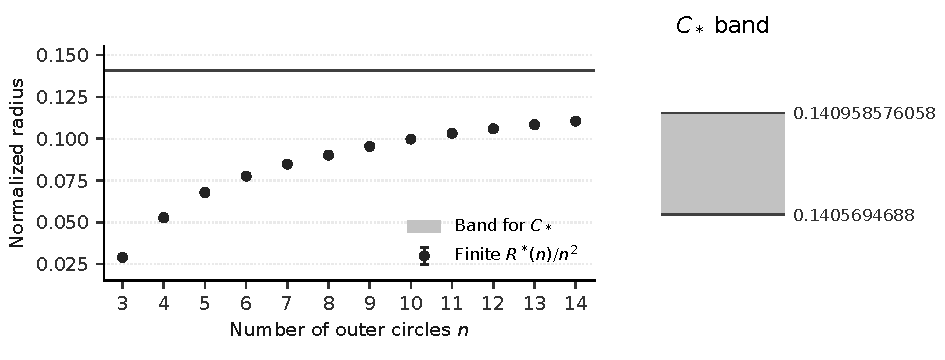
\includegraphics[width=.95\linewidth]{figures/finite_brackets.pdf}
\caption{Certified brackets for $\Rstar(n)/n^2$ from Paper~I
\cite{paperI}. Each interval has width $10^{-11}/n^2$, smaller than
its marker. The band between $\CstarLower$ and $\CstarUpper$ encloses the
limiting coefficient $\CC$. The right panel enlarges the band.}
\label{fig:finite}
\end{figure}

Sharper endpoint constructions, tractable evaluation of the finite
linear programs, the structure of optimizing orders and subleading
terms remain open. Bounds on the limiting coefficient alone place
no contact requirements on an individual finite optimizer.\label{page:main-end}

\section*{Data and code availability}

Supplement S1 gives the proof and exact verifier for
Proposition~\ref{prop:lower}. In the
\href{https://github.com/falker47/ringmin/raw/4b3721df8061f1992cfd242df69b1a0643216d8f/paper_assets/paper_ii_journal/source_bundle.zip}{frozen archive}
run \texttt{python -I -S verify.py} from \texttt{lower\_supplement/}.
The \href{https://github.com/falker47/ringmin/tree/eb9467dfa1429d622402e26e2f33017f984d2b1f/paper_assets/line_upper}{line-certificate package}
contains both witnesses and the four-block cost calculation. From
\texttt{paper\_assets/line\_upper/} run
{\small
\begin{verbatim}
python -I -S verify_line_certificate.py certificates/p1_n03200.json
python -I -S verify_line_certificate.py certificates/p2_n03200.json
\end{verbatim}
}
Each command checks the permutation, the span, all $5\,118\,400$ pairs and
the strict ceiling using the Python standard library.

\section*{Acknowledgment}
AI assistance was used for proof exploration, software, drafting and
adversarial checks. Responsibility for the mathematical statements and
presentation rests with the author.
% author: add Claude (Anthropic) to this statement

\clearpage
\bibliographystyle{siamplain}
\bibliography{references}
\end{document}
